% This file was converted to LaTeX by Writer2LaTeX ver. 1.0.2
% see http://writer2latex.sourceforge.net for more info
\documentclass[twoside,letterpaper]{article}
\usepackage[latin1]{inputenc}
\usepackage[T1]{fontenc}
\usepackage[english]{babel}
\usepackage{amsmath}
\usepackage{amssymb,amsfonts,textcomp}
\usepackage{color}
\usepackage{array}
\newcolumntype{M}[1]{>{\centering\arraybackslash}m{#1}}
\usepackage{supertabular}
\usepackage{hhline}
\usepackage{hyperref}
\usepackage{float}
\hypersetup{pdftex, colorlinks=true, linkcolor=blue, citecolor=blue, filecolor=blue, urlcolor=blue, pdftitle=SOFTWARE DESIGN DOCUMENT (SRS), pdfauthor=Shaylyn Adams}
\usepackage[pdftex]{graphicx}
% Outline numbering
\setcounter{secnumdepth}{5}
\renewcommand\thesection{\arabic{section}}
\renewcommand\thesubsection{\arabic{section}.\arabic{subsection}}
\renewcommand\thesubsubsection{\arabic{section}.\arabic{subsection}.\arabic{subsubsection}}
\renewcommand\theparagraph{\arabic{section}.\arabic{subsection}.\arabic{subsubsection}.\arabic{paragraph}}
\renewcommand\thesubparagraph{\arabic{section}.\arabic{subsection}.\arabic{subsubsection}.\arabic{paragraph}.\arabic{subparagraph}}
\makeatletter
\newcommand\arraybslash{\let\\\@arraycr}
\makeatother
% Page layout (geometry)
\setlength\voffset{-1in}
\setlength\hoffset{-1in}
\setlength\topmargin{0.5in}
\setlength\oddsidemargin{1in}
\setlength\evensidemargin{1in}
\setlength\textheight{8.278in}
\setlength\textwidth{6.5in}
\setlength\footskip{0.561in}
\setlength\headheight{0.5in}
\setlength\headsep{0.461in}
% Footnote rule
\setlength{\skip\footins}{0.0469in}
\renewcommand\footnoterule{\vspace*{-0.0071in}\setlength\leftskip{0pt}\setlength\rightskip{0pt plus 1fil}\noindent\textcolor{black}{\rule{0.25\columnwidth}{0.0071in}}\vspace*{0.0398in}}
% Pages styles
\makeatletter
\newcommand\ps@Standard{
  \renewcommand\@oddhead{\selectlanguage{english}\rmfamily\color{black} University of Massachusetts CICS \hfill \hfill Health-e}
  \renewcommand\@evenhead{\@oddhead}
  \renewcommand\@oddfoot{\foreignlanguage{english}{\textcolor{black}{SRS Page }}\foreignlanguage{english}{\textcolor{black}{\thepage{}}}}
  \renewcommand\@evenfoot{\@oddfoot}
  \renewcommand\thepage{\arabic{page}}
}
\newcommand\ps@Convertviii{
  \renewcommand\@oddhead{}
  \renewcommand\@evenhead{\@oddhead}
  \renewcommand\@oddfoot{}
  \renewcommand\@evenfoot{\@oddfoot}
  \renewcommand\thepage{\arabic{page}}
}
\newcommand\ps@Convertvii{
  \renewcommand\@oddhead{}
  \renewcommand\@evenhead{\@oddhead}
  \renewcommand\@oddfoot{}
  \renewcommand\@evenfoot{\@oddfoot}
  \renewcommand\thepage{\arabic{page}}
}
\newcommand\ps@Convertvi{
  \renewcommand\@oddhead{}
  \renewcommand\@evenhead{\@oddhead}
  \renewcommand\@oddfoot{}
  \renewcommand\@evenfoot{\@oddfoot}
  \renewcommand\thepage{\arabic{page}}
}
\newcommand\ps@Convertv{
  \renewcommand\@oddhead{}
  \renewcommand\@evenhead{\@oddhead}
  \renewcommand\@oddfoot{}
  \renewcommand\@evenfoot{\@oddfoot}
  \renewcommand\thepage{\arabic{page}}
}
\newcommand\ps@Convertiv{
  \renewcommand\@oddhead{}
  \renewcommand\@evenhead{\@oddhead}
  \renewcommand\@oddfoot{}
  \renewcommand\@evenfoot{\@oddfoot}
  \renewcommand\thepage{\arabic{page}}
}
\newcommand\ps@Convertii{
  \renewcommand\@oddhead{}
  \renewcommand\@evenhead{\@oddhead}
  \renewcommand\@oddfoot{}
  \renewcommand\@evenfoot{\@oddfoot}
  \renewcommand\thepage{\arabic{page}}
}
\newcommand\ps@FirstPage{
  \renewcommand\@oddhead{}
  \renewcommand\@evenhead{\@oddhead}
  \renewcommand\@oddfoot{}
  \renewcommand\@evenfoot{\@oddfoot}
  \renewcommand\thepage{\arabic{page}}
}
\makeatother
\pagestyle{Standard}
\setlength\tabcolsep{1mm}
\renewcommand\arraystretch{1.3}
% footnotes configuration
\makeatletter
\renewcommand\thefootnote{\arabic{footnote}}
\makeatother
\begin{document}
\clearpage\setcounter{page}{1}\pagestyle{Standard}
\thispagestyle{FirstPage}
\clearpage{\centering\selectlanguage{english}\bfseries\color{black}
SOFTWARE DESIGN DOCUMENT (SDD) FOR 
\par}


\bigskip

{\centering\selectlanguage{english}\bfseries\color{black}
320 Green Team Project
\par}


\bigskip


\begin{figure}
\centering

\includegraphics[width=1.5in,height=1.5in]{Uma_seal.png}
\end{figure}

\bigskip


\bigskip

{\centering\selectlanguage{english}\bfseries\color{black}
Version 1.0
\par}

{\centering\selectlanguage{english}\bfseries\color{black}
November 8, 2015
\par}


\bigskip


\bigskip

{\centering\selectlanguage{english}\bfseries\color{black}
Prepared for:
\par}

{\centering\selectlanguage{english}\bfseries\color{black}
Sunderland/Leverett, MA Health Inspector
\par}


\bigskip


\bigskip

{\centering\selectlanguage{english}\bfseries\color{black}
Prepared by:
\par}

{\centering\selectlanguage{english}\bfseries\color{black}
Ather Akhtar, Andrew Chang, Peter Marathas, Andrew Marchetti, \par} 
{\centering\selectlanguage{english}\bfseries\color{black}
 Michael Markman, Eric Maryea, Neven Recchia,
\par}
{\centering\selectlanguage{english}\bfseries\color{black}
Shawn Sowersby, Alex Sullivan, and Josh Tranfaglia.\par}

{\centering\selectlanguage{english}\bfseries\color{black}
University of Massachusetts
\par}

{\centering\selectlanguage{english}\bfseries\color{black}
Amherst, MA \ 01003
\par}


\clearpage{\centering\selectlanguage{english}\bfseries\color{black}
\foreignlanguage{english}{\MakeUppercase{\ }}\foreignlanguage{english}{\MakeUppercase{320 
Green Team Project: Health-e}}
\par}

{\centering\selectlanguage{english}\bfseries\color{black}
TABLE OF CONTENTS
\par}


\bigskip

{\selectlanguage{english}\bfseries\color{black}
Section\ \hfill  Page}

\setcounter{tocdepth}{9}
\renewcommand\contentsname{}
\tableofcontents

\bigskip

\clearpage\clearpage\setcounter{page}{1}\pagestyle{Convertii}
\section[INTRODUCTION]{\selectlanguage{english}\rmfamily\bfseries\color{black}
INTRODUCTION}

\subsection[Goals and Objectives]{\selectlanguage{english}\rmfamily\bfseries\color{black}
GOALS AND OBJECTIVES}
{\selectlanguage{english}\rmfamily\color{black}
Introduction to design document.
}

\subsubsection[Browsing and Search]{\selectlanguage{english}\rmfamily\bfseries\color{black}
Browsing and Search}
{\selectlanguage{english}\rmfamily\color{black}
Introduction to design document.
}
\subsubsection[Form Entry]{\selectlanguage{english}\rmfamily\bfseries\color{black}
Browsing and Search}
{\selectlanguage{english}\rmfamily\color{black}
Introduction to design document.
}
\subsubsection[Delayed Upload]{\selectlanguage{english}\rmfamily\bfseries\color{black}
Browsing and Search}
{\selectlanguage{english}\rmfamily\color{black}
Introduction to design document.
}

\subsection[Project Overview and Scope]{\selectlanguage{english}\rmfamily\bfseries\color{black}
Project Overview and Scope}
{\selectlanguage{english}\rmfamily\color{black}
WRITE HERE}
\newline
\begin{flushleft}
\tablehead{}
\begin{supertabular}{|m{1.3587599in}|m{5.00806in}|}
\hline
\centering \selectlanguage{english}\bfseries\color{black} Term or
Acronym &
\centering\arraybslash \selectlanguage{english}\bfseries\color{black}
Definition\\\hline
\selectlanguage{english}\color{black} Alpha test &
\selectlanguage{english}\color{black} Limited release(s) to selected,
outside testers\\\hline
\selectlanguage{english}\color{black} Beta test &
\selectlanguage{english}\color{black} Limited release(s) to cooperating
customers wanting early access to developing systems\\\hline
\selectlanguage{english}\color{black} Final test &
\selectlanguage{english}\color{black} aka, Acceptance test, release of
full functionality to customer for approval\\\hline
\selectlanguage{english}\color{black} DFD &
\selectlanguage{english}\color{black} Data Flow Diagram\\\hline
\selectlanguage{english}\color{black} SDD &
\selectlanguage{english}\color{black} Software Design Document, aka SDS,
Software Design Specification\\\hline
\selectlanguage{english}\color{black} SRS &
\selectlanguage{english}\color{black} Software Requirements
Specification\\\hline
\selectlanguage{english}\color{black} SSRS &
\selectlanguage{english}\color{black} System and Software Requirements
Specification\\\hline
~
 &
~
\\\hline
~
 &
~
\\\hline
~
 &
~
\\\hline
~
 &
~
\\\hline
\end{supertabular}
\end{flushleft}

% \subsection[REFERENCESS]{\selectlanguage{english}\rmfamily\bfseries\color{black}
% REFERENCES}
% {\selectlanguage{english}\itshape\color{black}
% WRITE HERE}
\clearpage\section[CORE FEATURES]{\selectlanguage{english}\rmfamily\bfseries\color{black}
SYSTEM OVERVIEW}

\clearpage\section[ADDITIONAL FEATURES]{\selectlanguage{english}\rmfamily\bfseries\color{black}
SYSTEM OVERVIEW}

\subsection[Software Context]{\selectlanguage{english}\rmfamily\bfseries\color{black}
Software Context}
{\selectlanguage{english}\rmfamily\color{black}
WRITE HERE}
\subsection[Major Constraints]{\selectlanguage{english}\rmfamily\bfseries\color{black}
Major Constraints}
{\selectlanguage{english}\rmfamily\color{black}
WRITE HERE}
\subsection[Intended Audience and Reading Suggestions]{\selectlanguage{english}\rmfamily\bfseries\color{black}
Intended Audience and Reading Suggestions}
{\selectlanguage{english}\rmfamily\color{black}
WRITE HERE}

\begin{figure}[H]
\centering
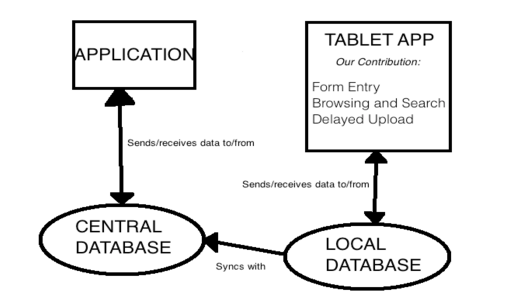
\includegraphics[width=4in,height=3in]{Diagram1.png}
\end{figure}




\clearpage\section[DATA DESIGN]{\selectlanguage{english}\rmfamily\bfseries\color{black}
DATA DESIGN}
\subsection[Internal Software Data Structure]{\selectlanguage{english}\rmfamily\bfseries\color{black}
Internal Software Data Structure}
{\selectlanguage{english}\rmfamily\color{black}
WRITE HERE}
\subsection[Global Data Structure]{\selectlanguage{english}\rmfamily\bfseries\color{black}
Global Data Structure}
{\selectlanguage{english}\rmfamily\color{black}
WRITE HERE}
\subsection[Temporary Data Structure]{\selectlanguage{english}\rmfamily\bfseries\color{black}
Temporary Data Structure}
{\selectlanguage{english}\rmfamily\color{black}
WRITE HERE}
\subsection[Database Description]{\selectlanguage{english}\rmfamily\bfseries\color{black}
Database Description}
{\selectlanguage{english}\rmfamily\color{black}
WRITE HERE}

\clearpage\section[ARCHITECTURAL AND COMPONENT-LEVEL DESIGN]{\selectlanguage{english}\rmfamily\bfseries\color{black}
ARCHITECTURAL AND COMPONENT-LEVEL DESIGN}
\subsection[System Structure]{\selectlanguage{english}\rmfamily\bfseries\color{black}
System Structure}

\subsubsection[Browsing and Search]{\selectlanguage{english}\rmfamily\bfseries\color{black}
Browsing and Search}
{\selectlanguage{english}\rmfamily\color{black}
Introduction to design document.
}
\subsubsection[Form Entry]{\selectlanguage{english}\rmfamily\bfseries\color{black}
Browsing and Search}
{\selectlanguage{english}\rmfamily\color{black}
Introduction to design document.
}
\subsubsection[Delayed Upload]{\selectlanguage{english}\rmfamily\bfseries\color{black}
Browsing and Search}
{\selectlanguage{english}\rmfamily\color{black}
Introduction to design document.
}

{\selectlanguage{english}\rmfamily\color{black}
Write Here
}
\subsection[BEGIN DEFINING SUB CLASSES...]{\selectlanguage{english}\rmfamily\bfseries\color{black}
BEGIN DEFINING SUB CLASSES...}
{\selectlanguage{english}\rmfamily\color{black}
Write Here
}



%\clearpage\section[DATA MODELING]{\selectlanguage{english}\rmfamily\bfseries\color{black}
%DATA MODELING}

\clearpage\section{User Interface Design}

\subsection[Description of the User Interface]{\selectlanguage{english}\rmfamily\bfseries\color{black}
Description of the User Interface}
{\selectlanguage{english}\rmfamily\color{black}
Describethefunctionality of thesystem from the users perspective. Explain howtheuser
will be able to use your system to complete all the expected features and the feedback
information that will bedisplayedfor theuser.
}

\subsubsection[Browsing and Search]{\selectlanguage{english}\rmfamily\bfseries\color{black}
Browsing and Search}
{\selectlanguage{english}\rmfamily\color{black}
Introduction to design document.
}
\subsubsection[Form Entry]{\selectlanguage{english}\rmfamily\bfseries\color{black}
Browsing and Search}
{\selectlanguage{english}\rmfamily\color{black}
Introduction to design document.
}
\subsubsection[Delayed Upload]{\selectlanguage{english}\rmfamily\bfseries\color{black}
Browsing and Search}
{\selectlanguage{english}\rmfamily\color{black}
Introduction to design document.
}

\subsection[For first time users]{\selectlanguage{english}\rmfamily\bfseries\color{black}
For first time users}
{\selectlanguage{english}\rmfamily\color{black}
Describethefunctionality of thesystem from the users perspective. Explain howtheuser
will be able to use your system to complete all the expected features and the feedback
information that will bedisplayedfor theuser.
}
\subsection[For returning users]{\selectlanguage{english}\rmfamily\bfseries\color{black}
For first time users}
{\selectlanguage{english}\rmfamily\color{black}
Describethefunctionality of thesystem from the users perspective. Explain howtheuser
will be able to use your system to complete all the expected features and the feedback
information that will bedisplayedfor theuser.
}
\subsection[Screen Images]{\selectlanguage{english}\rmfamily\bfseries\color{black}
Screen Images}
{\selectlanguage{english}\rmfamily\color{black}
Display screenshots showingtheinterfacefrom theusers perspective. Thesecan be handdrawn
or youcan use an automateddrawing tool. Just make them as accurateas possible.
(Graph paper workswell.)
}
\subsection[Screen Objects and Actions]{\selectlanguage{english}\rmfamily\bfseries\color{black}
Screen Objects and Actions}
{\selectlanguage{english}\rmfamily\color{black}
A discussion of screen objects andactions associatedwith thoseobjects.
}

\clearpage\section[Restrictions Limitations and Constraints ]{\selectlanguage{english}\rmfamily\bfseries\color{black}
Restrictions Limitations and Constraints}

\clearpage\section[Testing Issues ]{\selectlanguage{english}\rmfamily\bfseries\color{black}
Testing Issues}

\subsection[Testing cases and expected results]{\selectlanguage{english}\rmfamily\bfseries\color{black}
Testing cases and expected results}
{\selectlanguage{english}\rmfamily\color{black}
A discussion of screen objects andactions associatedwith thoseobjects.
}
\subsection[Performance Bounds]{\selectlanguage{english}\rmfamily\bfseries\color{black}
Performance Bounds}
{\selectlanguage{english}\rmfamily\color{black}
A discussion of screen objects andactions associatedwith thoseobjects.
}
\subsection[Critical Systems]{\selectlanguage{english}\rmfamily\bfseries\color{black}
Critical Systems}
{\selectlanguage{english}\rmfamily\color{black}
A discussion of screen objects andactions associatedwith thoseobjects.
}
\subsection[Testing Cases]{\selectlanguage{english}\rmfamily\bfseries\color{black}
Testing Cases}
{\selectlanguage{english}\rmfamily\color{black}
A discussion of screen objects andactions associatedwith thoseobjects.
}

\clearpage\section[APPENDIX A. ]{\selectlanguage{english}\rmfamily\bfseries\color{black}
APPENDIX A. \ Example Screens}

\bigskip

{\selectlanguage{english}\itshape\color{black}
Include copies of specifications, mockups, prototypes, etc. supplied or
derived from the customer. \ Appendices are labeled A, B, {\dots}n.
\ \ Reference each appendix as appropriate in the text of the document.
}

{\selectlanguage{english}\color{black}
\foreignlanguage{english}{\ }\foreignlanguage{english}{[ insert appendix
A here ]}}




\bigskip
\end{document}
